\begin{frame}{The $\Upsilon$ fit model}
\setlength{\unitlength}{1mm}
\begin{columns}
\column{.5\textwidth}
\scalebox{0.7}{
  \begin{picture}(75,60)
    \put(0,0){
      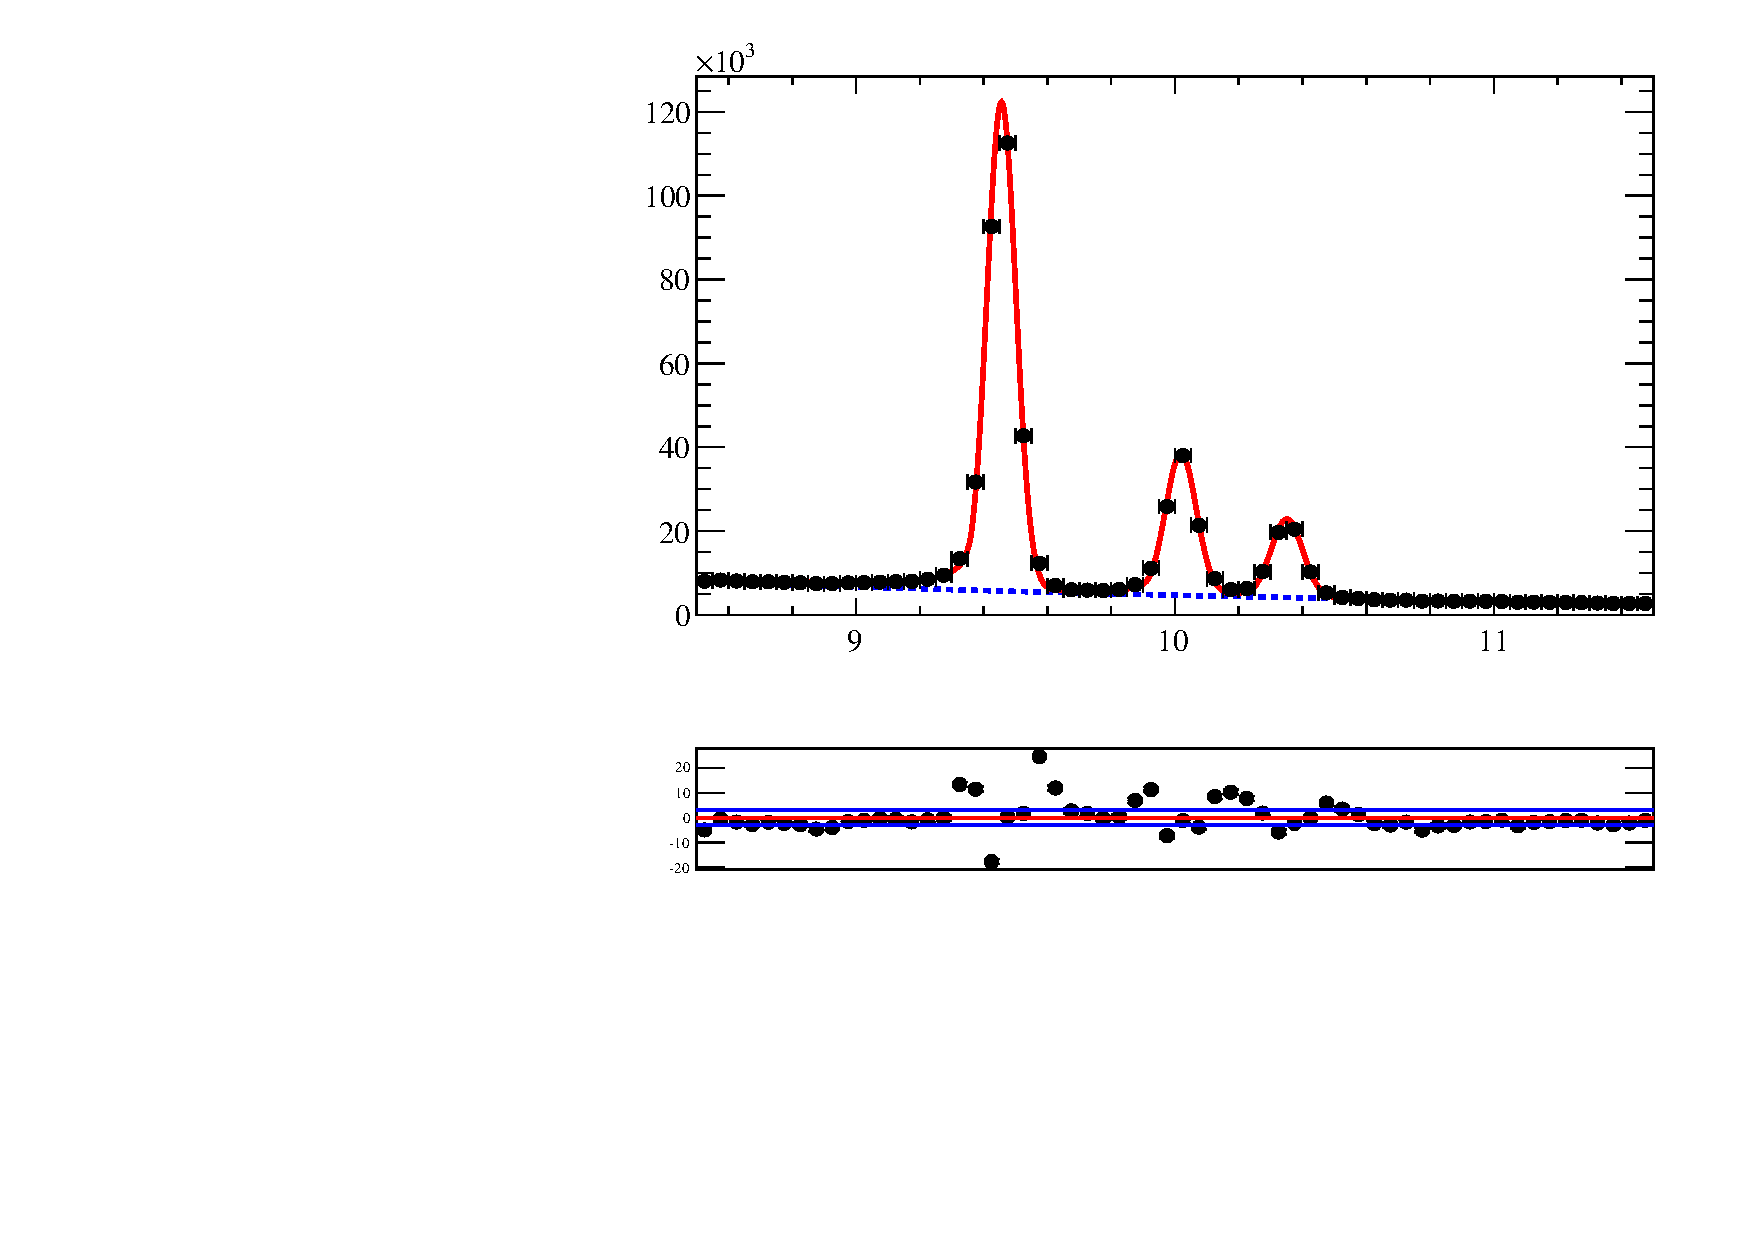
\includegraphics[width=75mm, height=60mm]{upsilon-fit/f2011_6_40}
    }
    \put(0,18){\small \begin{sideways}Candidates/(40\mevcc)\end{sideways}}
    \put(25, 0){$m_{\mumu} \left[\gevcc\right]$}
    \put(45,45){\sqs = 7 \tev}
    \put(35,38){$6 < p_T^{\mumu} < 40 \gevc$}
    % \graphpaper[5](0,0)(150, 60)
  \end{picture}
}
\begin{itemize}
\item 3 Double Crystal Ball functions for signal yields.
\item Exponential function for combinatorial background.
\end{itemize}

\column{.5\textwidth}
\resizebox{.75\textwidth}{!}{
\begin{tabular}{lrr}\toprule
 & \multicolumn{2}{c}{$\mumu$ transverse momentum intervals, \gevc}\\
 & \multicolumn{2}{c}{6 -- 40}\\
\cmidrule(r){2-3}
 & \multicolumn{1}{c}{\sqs = 7\tev} & \multicolumn{1}{c}{\sqs = 8\tev}\\
\midrule
$N_{\Y1S}$ & 283,300 $\pm$ 600 & 659,600 $\pm$ 900\\
$N_{\Y2S}$ & 87,500 $\pm$ 400 & 203,300 $\pm$ 600\\
$N_{\Y3S}$ & 50,420 $\pm$ 290 & 115,300 $\pm$ 400\\

\rule{0pt}{4ex}Background & 296,400 $\pm$ 700 & 721,300 $\pm$ 1100\\

\rule{0pt}{4ex}$\mu_{\Y1S}, \mevcc$ & 9457.02 $\pm$ 0.10 & 9455.58 $\pm$ 0.07\\
$\sigma_{\Y1S}, \mevcc$ & 42.86 $\pm$ 0.10 & 43.04 $\pm$ 0.06\\

\rule{0pt}{4ex}$\mu_{\Y2S}, \mevcc$ & 10,019.03 $\pm$ 0.21 & 10,018.05 $\pm$ 0.14\\
$\sigma_{\Y2S}, \mevcc$ & 46.38 $\pm$ 0.20 & 46.45 $\pm$ 0.14\\

\rule{0pt}{4ex}$\mu_{\Y3S}, \mevcc$ & 10,351.16 $\pm$ 0.32 & 10,349.41 $\pm$ 0.16\\
$\sigma_{\Y3S}, \mevcc$ & 48.63 $\pm$ 0.31 & 48.24 $\pm$ 0.11\\

$\tau$ & -0.3887 $\pm$ 0.0023 & -0.3819 $\pm$ 0.0015\\
\bottomrule
\end{tabular}
} % scalebox

\bigskip

\begin{itemize}
\item \Y1S mass is about 5 \mevcc lower than PDG value $9460.30 \pm  0.26$ \mevcc
% \item In this study \OneS mass was fixed to $9.456 \gevcc$ 
\end{itemize}
\end{columns}


\end{frame}

